 %%%%%%%%%%%%%%%%%%%%%%%%%%%%%%%%%%%%%%%%%
% Short Sectioned Assignment
% LaTeX Template
% Version 1.0 (5/5/12)
%
% This template has been downloaded from:
% http://www.LaTeXTemplates.com
%
% Original author:
% Frits Wenneker (http://www.howtotex.com)
%
% License:
% CC BY-NC-SA 3.0 (http://creativecommons.org/licenses/by-nc-sa/3.0/)
%
%%%%%%%%%%%%%%%%%%%%%%%%%%%%%%%%%%%%%%%%%

%----------------------------------------------------------------------------------------
%   PACKAGES AND OTHER DOC%%UMENT CONFIGURATIONS
%----------------------------------------------------------------------------------------

\documentclass[paper=a4, fontsize=11pt]{scrartcl} % A4 paper and 11pt font size

%\usepackage[final]{pdfpages}
\usepackage[utf8]{inputenc}
\usepackage[T1]{fontenc} % Use 8-bit encoding that has 256 glyphs
%\usepackage{fourier} % Use the Adobe Utopia font for the document - comment this line to return to the LaTeX default
\usepackage[polish]{babel} % English language/hyphenation
\usepackage{amsmath,amsfonts,amsthm} % Math packages

\usepackage[usenames,dvipsnames]{color} % Required for custom colors
\usepackage{graphicx}
\usepackage{caption}
\usepackage{subcaption}
\usepackage{listings} % Required for insertion of code

\usepackage{lastpage}
\usepackage{tabularx}

%\usepackage{todonotes}

\usepackage{sectsty} % Allows customizing section commands
\allsectionsfont{ \normalfont\scshape} % Make all sections the default font and small caps

\usepackage{fancyhdr} % Custom headers and footers
\pagestyle{fancyplain} % Makes all pages in the document conform to the custom headers and footers
\fancyhead{} % No page header - if you want one, create it in the same way as the footers below
\fancyfoot[L]{} % Empty left footer
\fancyfoot[C]{} % Empty center footer
\fancyfoot[R]{\thepage \, z \pageref{LastPage}} % Page numbering for right footer
\renewcommand{\headrulewidth}{0pt} % Remove header underlines
\renewcommand{\footrulewidth}{0pt} % Remove footer underlines
\setlength{\headheight}{6.6pt} % Customize the height of the header



\numberwithin{equation}{section} % Number equations within sections (i.e. 1.1, 1.2, 2.1, 2.2 instead of 1, 2, 3, 4)
\numberwithin{figure}{section} % Number figures within sections (i.e. 1.1, 1.2, 2.1, 2.2 instead of 1, 2, 3, 4)
\numberwithin{table}{section} % Number tables within sections (i.e. 1.1, 1.2, 2.1, 2.2 instead of 1, 2, 3, 4)

%\setlength\parindent{0pt} % Removes all indentation from paragraphs - comment this line for an assignment with lots of text

%----------------------------------------------------------------------------------------
%   CODE INCLUSION CONFIGURATION
%----------------------------------------------------------------------------------------

\definecolor{MyDarkGreen}{rgb}{0.0,0.4,0.0} % This is the color used for comments
\lstloadlanguages{C++} % Load Cpp syntax for listings, for a list of other languages supported see: ftp://ftp.tex.ac.uk/tex-archive/macros/latex/contrib/listings/listings.pdf
\lstset{language=C++, % UseCpp
        frame=single, % Single frame around code
        basicstyle=\small\ttfamily, % Use small true type font
        keywordstyle=[1]\color{Blue}\bf, % Perl functions bold and blue
        keywordstyle=[2]\color{Purple}, % Perl function arguments purple
        keywordstyle=[3]\color{Blue}\underbar, % Custom functions underlined and blue
        identifierstyle=, % Nothing special about identifiers
        commentstyle=\usefont{T1}{pcr}{m}{sl}\color{MyDarkGreen}\small, % Comments small dark green courier font
        stringstyle=\color{Purple}, % Strings are purple
        showstringspaces=false, % Don't put marks in string spaces
        tabsize=5, % 5 spaces per tab
        %
        % Put standard Perl functions not included in the default language here
        morekeywords={rand},
        %
        % Put Cppl function parameters here
        morekeywords=[2]{on, off, interp},
        %
        % Put user defined functions here
        morekeywords=[3]{test},
        %
        morecomment=[l][\color{Blue}]{...}, % Line continuation (...) like blue comment
        numbers=left, % Line numbers on left
        firstnumber=1, % Line numbers start with line 1
        numberstyle=\tiny\color{Blue}, % Line numbers are blue and small
        stepnumber=5 % Line numbers go in steps of 5
}

% add new command to include cpp code
\newcommand{\cppscript}[2]{
\begin{itemize}
\item[]\lstinputlisting[caption=#2,label=#1]{#1.cpp}
\end{itemize}

}

%----------------------------------------------------------------------------------------
%   TITLE SECTION
%----------------------------------------------------------------------------------------

\newcommand{\horrule}[1]{\rule{\linewidth}{#1}} % Create horizontal rule command with 1 argument of height

\title{
\vspace*{\fill}
\normalfont
\textsc{Projekt Zespołowy}\\ [20pt]
\horrule{1.5pt} \\[0.4cm] % Thin top horizontal rule
\LARGE Baza danych szeregów czasowych implementowana na klastrze obliczeniowym procesorów graficznych
\horrule{1.5pt} \\[0.1cm] % Thick bottom horizontal rule
\normalsize
\textsc{Wstępna Specyfikacja Techniczna} \\ [20pt]
\vspace*{\fill}
}

\author{Jakub Dutkowski \\ Karol Dzitkowski \\ Tomasz Janiszewski } % Your name

\date{\normalsize\today} % Today's date or a custom date

\begin{document}
\maketitle

\thispagestyle{empty}
\clearpage

\tableofcontents
\listoffigures

\chapter{}

\clearpage

\vspace{4em}


\section{Abstrakt}
Niniejsza dokumentacja przedstawia wstępny opis techniczny systemu tworzonego w ramach projektu zespołowego, którego efektem ma być praca inżynierska.
Dokument zawiera powierzchowny opis struktury systemu od strony technicznej wraz z diagramami przepływu danych oraz wydzielonymi modułami systemu.

\section{Opis programu}
Celem projektu jest stworzenie bazy danych szeregów czasowych efektywnie korzystającej z wydajności oferowanej przez współczesne
procesory graficzne. Dane powinny być przechowywane i przetwarzane w pamięci kart graficznych. Baza danych oprócz przechowywania
danych powinna umożliwiać szybką ich agregację oraz filtrowanie.

\section{Ogólna wizja struktury systemu}
\begin{itemize}
	\item System będzie składał się z dwóch podsystemów:
		\begin{enumerate}
			\item Systemu serwera głównego zwanego Master
			\item Systemu działającego na serwerach bazodanowych - węzłach (Nodes)
		\end{enumerate}
	\item Komunikacja pomiędzy Masterem a węzłami odbywa się za pomocą tcp/ip po sieci wewnętrznej, gdzie informacje przesyłane są za pomocą 
		zserializowanych binarnie struktur danych. Klienci komunikują się tylko z Masterem który oferuje im Restowe api. 
	\item Dla klientów utworzone są serwisy:
		\begin{enumerate}
			\item Serwis danych (insertService)
				\begin{itemize}
					\item Insert (możliwe rozszerzenie o InsertMany)
					\item Flush
				\end{itemize}
			\item Serwis zapytań (queryService) - zawiera wszystkie zapytania typu select zawarte w "Specyfikacji Technicznej"
			\item Serwis statusu (statusService)
				\begin{itemize}
					\item GetLastError
				\end{itemize}
		\end{enumerate}
	\item Master zajmuje się odbieraniem zapytań od klientów, kolejkowaniem ich oraz zlecaniem ich wykonania przez węzły. Zarządza oraz monitoruje 
		węzły sprawdzając ich parametry, np. zajętość miejsca na karcie lub obciążenie. Nadzoruje wykonanie wszystkich zapytań oraz zbiera ich wyniki 
		wykonując na nich ostatni etap operacji Reduce (agregując wyniki). Gotowa odpowiedź na zapytanie kierowana jest z powrotem do klienta.
	\item Węzeł loguje się do Mastera jako gotowy do pracy węzeł. Zalogowany węzeł otrzymuje tyle identyfikatorów ile ma odpowiednich dla naszego systemu 
		(Cuda capability >= 2.0) kart graficznych NVIDIA. Główną rolą każdego węzła jest składowanie danych na kartach graficznych. Wykonują zlecane im 
		zadania (przez Mastera) wrzucając dane na odpowiednią kartę lub wykonując zapytanie na danych znajdujących się już na karcie. Takie dane mogą 
		być agregowane, sortowane oraz filtrowane na sposoby wymienione w "Specyfikacji Technicznej". W tym momencie kożystać będziemy z wydajności 
		kart graficznych. Węzeł komunikuje się tylko i wyłącznie z Masterem.
	
\end{itemize}




























































\begin{figure}
	\begin{center}
		\caption{Ogólna struktura systemu}
 		\makebox[\textwidth]{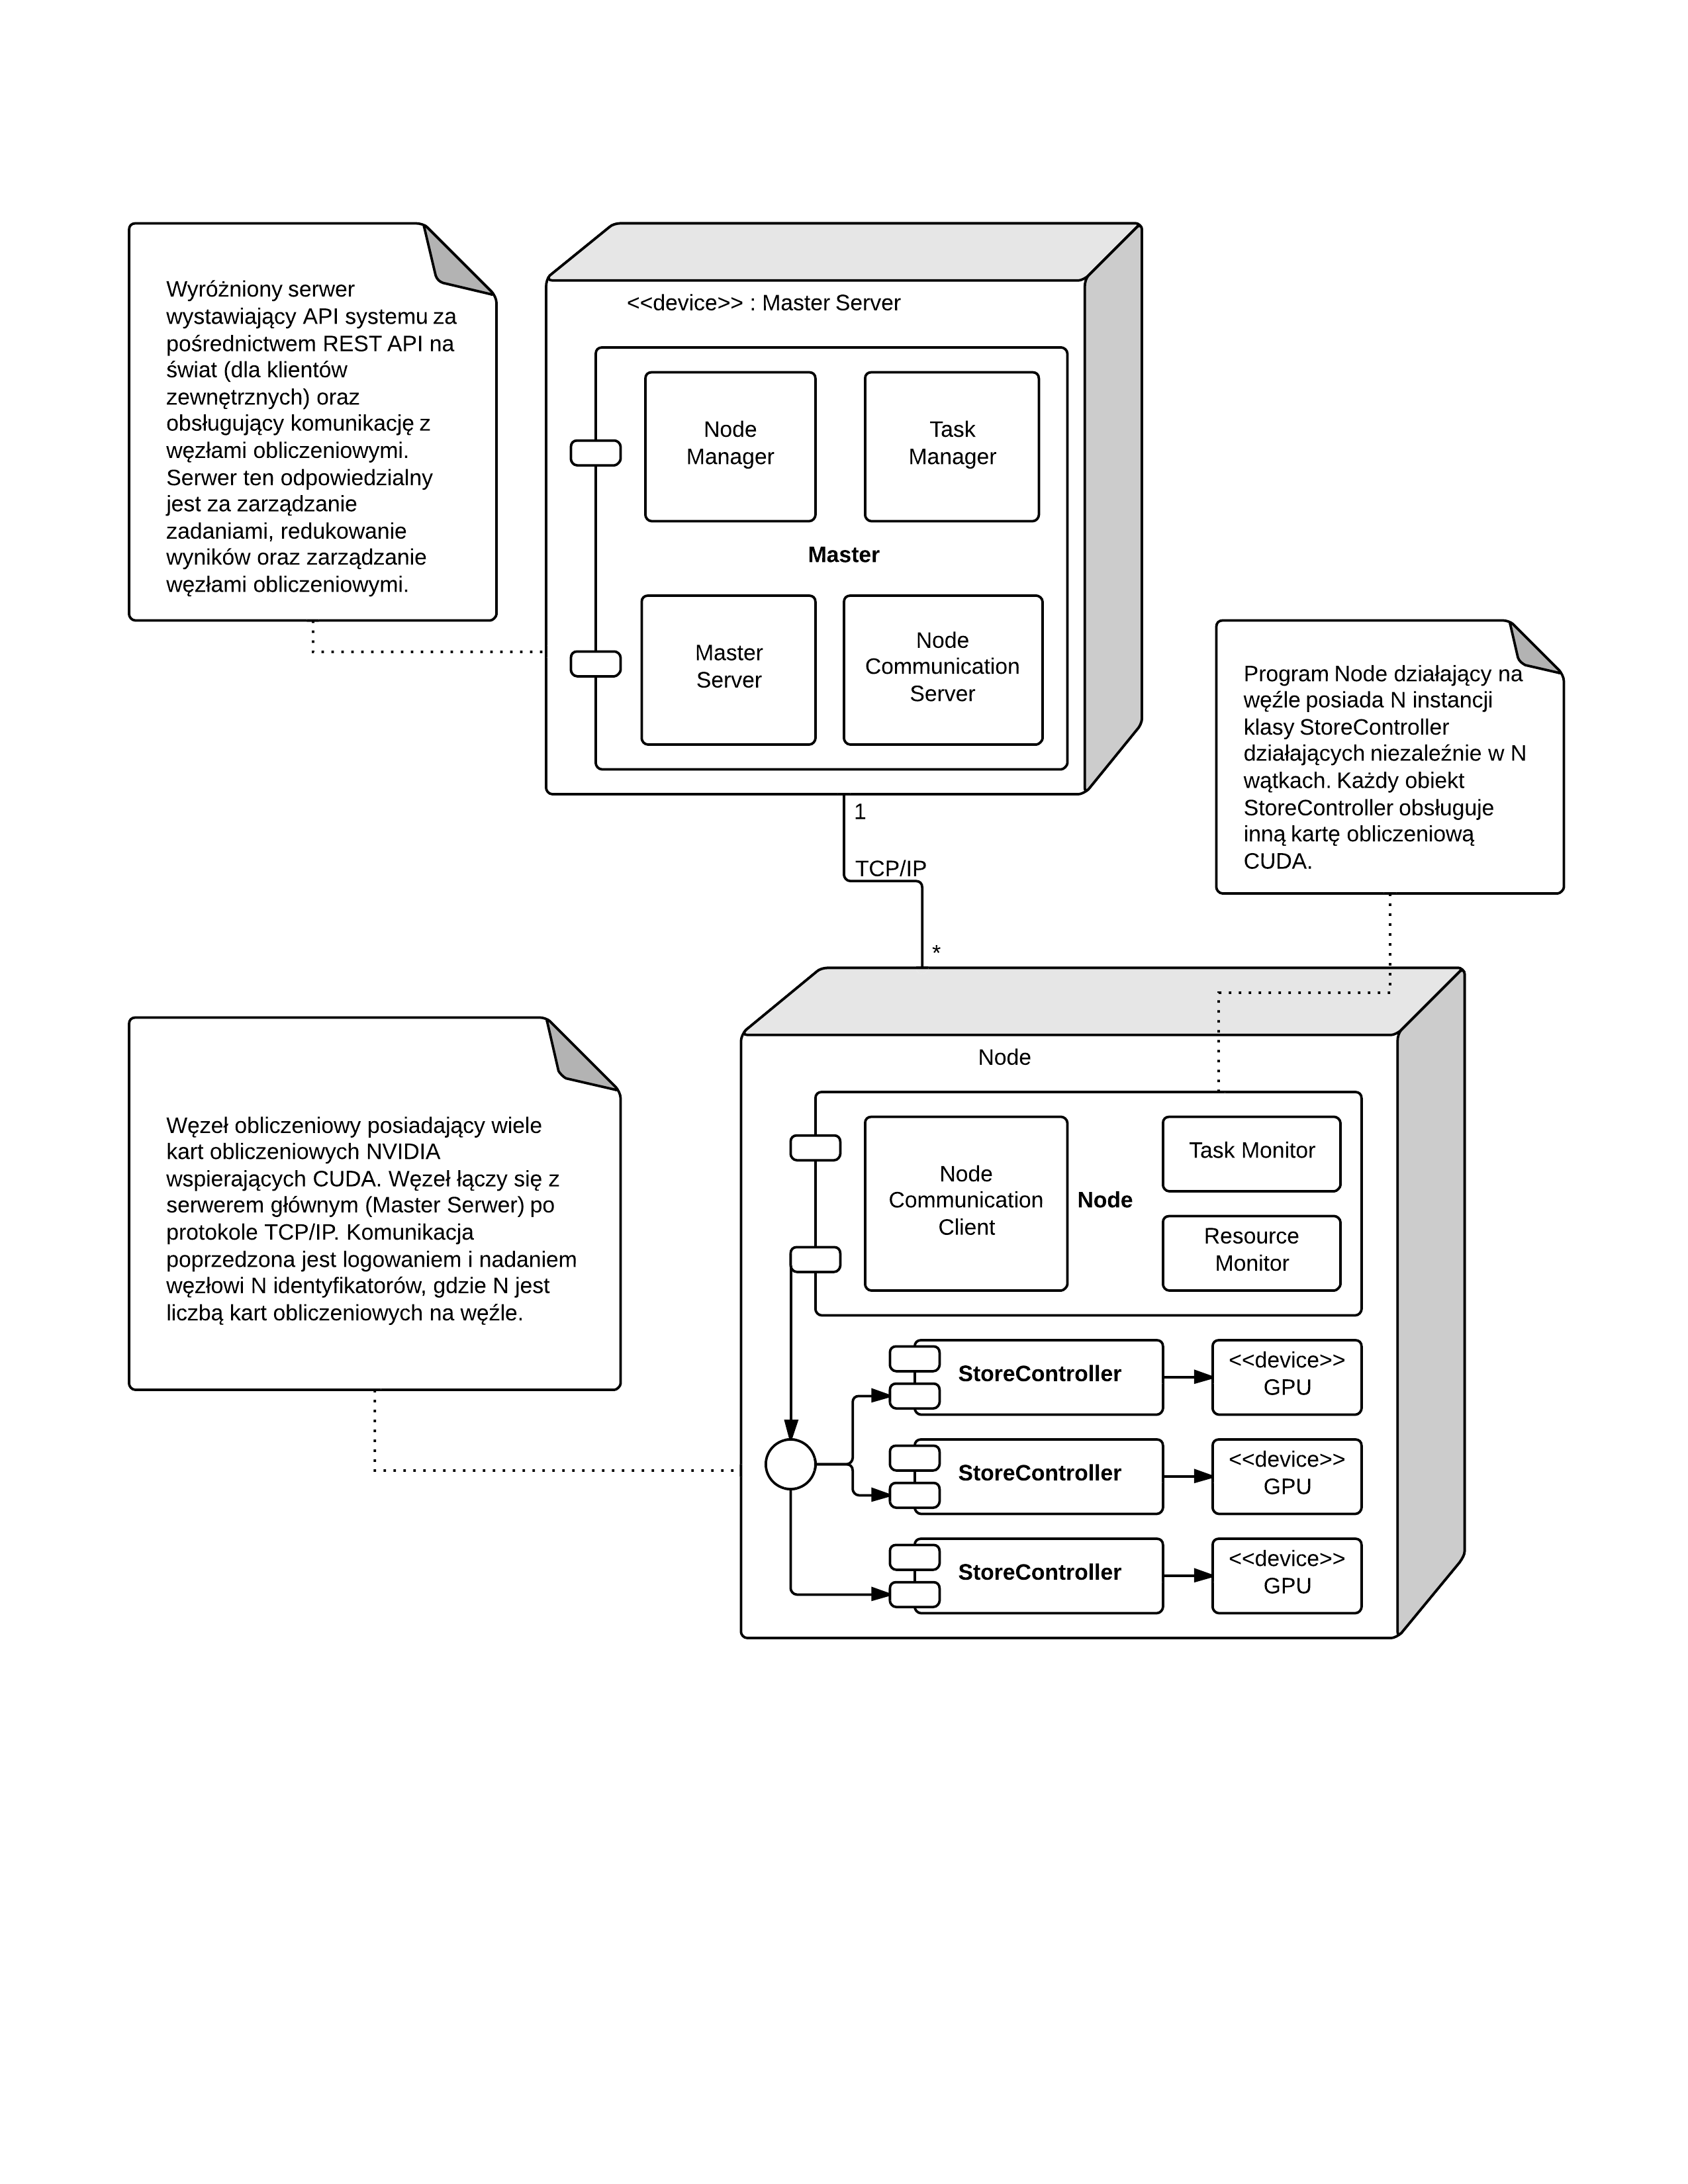
\includegraphics[width=\paperwidth]{Deployment_Diagram}}
	\end{center}
\end{figure}

\end{document}